
\documentclass[a4, 10pt,dvipdfmx,twocolumn]{jsarticle}

%\usepackage[chukan]{sotsuron}
%\usepackage[dvips]{graphicx}

%\setlength{\topmargin}{-13truemm}
%\setlength{\headheight}{0mm}
%\setlength{\headsep}{0mm}
%\setlength{\textheight}{45\baselineskip}
%\setlength{\textheight}{26cm}
%\addtolength{\textheight}{\topskip}
%\addtolength{\textwidth}{5cm}
%\addtolength{\oddsidemargin}{-2.5cm}

\usepackage[dvipdfmx]{graphicx}
\def\pgfsysdriver{pgfsys-dvipdfmx.def}
\usepackage{threeparttable}
\usepackage{tikz}
\usepackage[chukan, nobroaderlayout]{sotsuron}
% \usepackage[chukan]{sotsuron}
\usepackage{ascmac}
\usepackage{bm}
\usepackage{amsmath}
\usepackage{fancybox}
\usepackage{url}

\title{モンテカルロ木探索を用いた交渉の評価関数の提案}
\author{東京大学工学部電子情報学科 近山•鶴岡研究室 4年 伊藤 義章}
\date{2013年2月17日}

\begin{document}
 % \makecover

\pagenumbering{roman}

 % \tableofcontents

\newpage
\maketitle

\pagenumbering{arabic}

\section{目的と背景}

実世界では、競争的状況において自分の利益を最大化することを目指した多くの交渉が行なわれている。交渉に関する研究の多くは、交渉の定性的な研究であり、交渉の定量的な側面に着目した研究は未だ発展途上である。その理由のひとつは、交渉によって得られる可能性のある利益を数値化し、どのような交渉を提示するかの指標となる評価関数を用意することの難しさにある。本研究では、交渉において重要となる要素を定量的な観点から明らかにする事を目的とし、利益の数値化の方法として、行動の先読みおよび評価関数を用いる事を提案する。
具体的には、先読みによる利益計算に、近年成功をおさめているモンテカルロ法を用いることを提案し、また、利益計算の指標となる様々な評価関数を提示する。

\section{関連研究}
\subsection{UCTアルゴリズム (UCB applied to Trees)}
状態の評価が難しい問題において有効とされる手法としてモンテカルロ法がある。
ある局面から終局までランダムに行われる試行(プレイアウトと呼ばれる)に基づき、統計的に評価する。プレイアウトを繰り返す事で、ある局面の勝率を計算することができる。
しかし、有限な時間内に正確な勝率評価を行う場合、明らかに有望でない手に対して、有望な 手と同様の試行回数を行うべきではない。よって、これを解消するため有望な手にバイアスをかけて試行回数を配分する必要がある。これがUCBアルゴリズム (Upper Confidence Bound、以下 UCB) である\cite{kocsis2006bandit}。
子ノードを選択する場合、まず未探索の子ノードを優先的に選択する。
子ノードが全て探索済みの場合は、探索回数が少なく、高い報酬を得る可能
性のある手を優先的に選択する。
選択したノードをプレイアウトした後は、その結果を報酬として探索経路上のノードに更新する。
以上の「子ノードの選択」「子ノードの展開」「プレイアウト」「結果の更新」を終了条件 (時間や探索回数など) となるまで繰り返し、平均報酬の最も高い子ノードを次のアクションとする。
これらのアルゴリズムは、カタンのAIであるSettlersに適用させ、成功をおさめている\cite{szita2010monte}。JSettlersのプレイヤーに対して、JSettlersをベースとしたモンテカルロ木探索で、0回シミュレート、1000回シミュレートおよび10000回シミュレートを行った。他の3人プレイヤーに対し、25\%、27\%、49\% の勝率を残し、カタンにおけるモンテカルロ木探索がランダムプレイヤーよりは強いことを示している。
本研究でも、UCTアルゴリズムをSmartSettlersで適用するものとする。
% \begin{figure}[b]
%     \begin{center}
%       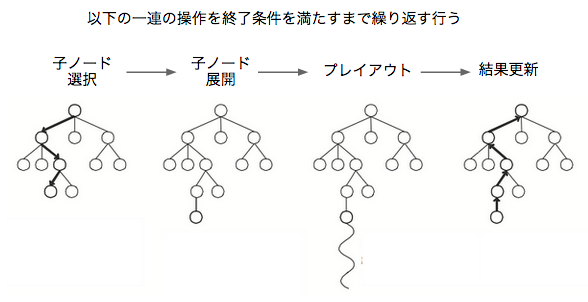
\includegraphics[width=80mm]{img/monte_carlo.png}
%     \end{center}
%     \caption{モンテカルロ木探索~\cite{kocsis2006bandit}}
%     \label{monte_carlo}
% \end{figure}

\subsection{交渉のアルゴリズム}
交渉を行なう場合、お互いの評価関数が異なっているため、自分の評価関数であれば受諾する交渉でも、相手の評価関数では受諾を選ばず、結果交渉が成立しないということがある。
交渉が決裂すると、実際に得られるはずだった利益を得られなくなることにより、機会損失を招いてしまう。そのため、交渉においてはお互いの妥協点をみつける必要がある。

妥協点を見つける方法として、相手のモデル化\cite{baarslag2012evaluating}がある。例えば、IAMhaggler2011は序盤の交渉でガウス過程的\cite{rasmussen2006gaussian}にモデル化を行なう事で、相手の利益を予測することができる。これを適用したIAMhaggler2011\cite{williams2013iamhaggler2011}とい人工知能は、ANAC(Automated Negotiating Agents Competition、以下ANAC)にて優秀な結果を残している。IAMhaggler2011は相手の利益を予測した後、自分の利益を最大化する交渉案が最もよい結果を残している。

また、交渉案を選択する評価関数の譲歩率を測定する方法\cite{baarslag2012evaluating}がある。譲歩率は機会損失をさける指標となる。
ANACにて優秀とされる結果を残した人工知能\cite{baarslag2012evaluating}は、一定の譲歩を行なっていることから、自分の利益のみを考える評価関数が優位な戦略でないと考えられる。

\section{提案手法}
\subsection{利益の見積もり}

UCTアルゴリズムによるプレイアウトによって、各プレイヤーの勝率を計算することができる。交渉による損得は最終的に自分の勝率に直結することから、UCTアルゴリズムの先読みによって予め得た勝率により利益計算を行なうことができると考えられる。よって、UCTアルゴリズムの先読みによって得た勝率を、利益計算に用いる事にする。 

\subsection{利益の見積もり}

本研究では、前節で得られた利益計算の結果を用いて、交渉の成功率を考慮した評価関数により交渉を提示する。
自分の利益を最大化しつつ、交渉の成功率をあげる必要がある。交渉の成功率は「相手が得られる利益」に影響を受けるものだと仮定する。
よって、良い交渉案を選ぶ評価関数として、以下の5つの評価方法を提案することにする。
まず、自分の利益のみしか考えない「自己中心的交渉」を行なうプレイヤーをベースラインとして扱う。次に、交渉の成功率よりも相手の利益を優先にした「利益優先交渉」と交渉の成功率を優先した「受諾優先交渉」を提示する。また、お互いの利益をバランスよく配分することで、自分の利益と交渉の成功率を調整する手法として「和交渉」「積交渉」を提示する。
\section{評価}
\subsection{UCTの利益計算}
結果より、ルールベースプレイヤーが全受諾プレイヤーに対して42.08\%(前述と同じ)と有意な実力差を残していることから、自分にとって有利となる利益計算を行い、交渉案を提示していることが分かる。一方で、UCTプレイヤーは受諾プレイヤーに対して23.55\%と25\%より低い勝率となった。すなわち、自分にとって有利な利益計算を行なうことができず、結果として有利な交渉案を提示できなかったと考えられる。
また、ランダムプレイヤーに対してもルールベースプレイヤーは41.25\%と高い勝率をおさめたが、UCTプレイヤーはランダムプレイヤーに対しても24.95\%と有意な実力差を得る事はできなかった。

図より、前述の通りプレイアウト回数が1,000回の方が100回よりも高い一致率となっている。また、いずれもルールベースよりも高い一致率になっていることがわかる。
また図より、勝率が高くなるほど、一致率が下がっていく傾向にある。プレイアウト回数が1,000回の場合では、相手プレイヤーの勝率が35\%以下の時に平均よりも高い一致率を示しているにも関わらず、勝率が90\%以上になると、プレイアウト回数が100回の一致率やランダムプレイヤーに近い一致率になってしまう。これは勝率が拮抗している序盤では良い交渉案を提示しているものの、勝率に差がついてくる終盤になると良い交渉案を選べない原因だと考えられる。相手の勝率が高くなってしまうと、良い交渉を提案できなくなる理由として、自分の勝率計算の精度が悪くなることが考えられる。全ての交渉案に対して1,000回のプレイアウトを行なうが、いずれの交渉案においても一度の交渉で大きく勝率が変わる事はないため、相手の勝率は90\%付近となっている。そのため、残りの10\%である100回のプレイアウト回数の中から良い交渉案を見つける必要があるが、プレイアウト回数を増やしたにも関わらず、良い一致率を得ることができなくなってしまう。よって、勝率計算において相手の勝率が高くなった場合には一定の重みをつけて計算することで、精度の悪化を防ぐ事が考えられ、今後の課題である。

以上より、UCTプレイヤーの勝率が受諾プレイヤー、ランダムプレイヤーに対して良い結果を残せなかった原因として、「プレイアウト回数が不十分であったこと」「相手の勝率が高くなった場合での精度悪化」が考えられるため、これらの改善を行なうことが課題となる。また、UCTプレイヤーよりもルールベースプレイヤーの方が良い結果を残した事から、ルールベースプレイヤーのほうが良い利益計算を行なっていると考え、交渉の評価選択手法を提案する上で、ルールベースプレイヤーを用いる事にする。



\subsection{評価関数}


\begin{figure}[t]
    \begin{center}
      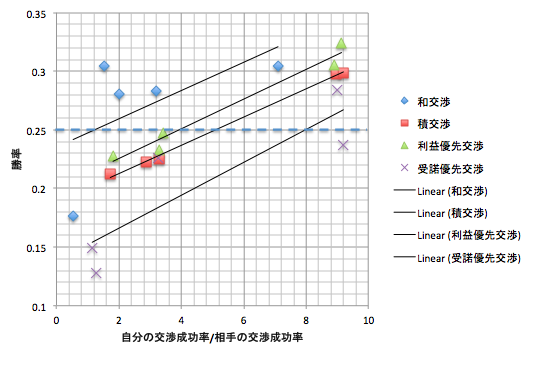
\includegraphics[width=120mm]{img/relation_winrate.png}
    \end{center}
    \caption{評価関数の勝率と交渉成功率}
    \label{win_rate}
\end{figure}




図より、全ての評価関数において(自分の交渉成功率/相手の交渉率)の割合が高まれば高まるほど良い勝率を残すことができると考えられる。このことからも、交渉における「提案成功率」と「受諾率」が関係していると考えられる。また、和交渉ではばらついたものの、利益優先交渉や、積交渉のように近似直線を描くと一定の直線上にのっていることがわかる。また、図よりこれら4つの直線の傾きは一定であるが、評価関数によってその近似直線が上下することがわかる。評価関数によって近似直線が上下する原因として、「自分にとっての利益」と「相手に与える損益」のバランスによるものと考えられる。バランス型の交渉である和交渉では、相手に与える損益を加えたことが高い勝率に結びついたと考えられる。また、受諾優先交渉、利益優先交渉と積交渉では相手に与える損益がないため、自分の得られる利益が大きい順に高い結果を残すことができたと考えられる。利益優先や受諾優先ではなくバランスよく利益配分を行なう和交渉がもっともよい結果を残したことから、「自分にとっての利益」と「相手に与える損益」をバランスよく配分する評価関数が最もよい評価関数だと考えられる。

また、相手プレイヤーによって受諾率や提案成功率が変化することから交渉において相手の評価関数に大きく影響をうけるものと考えられる。相手が楽観的な交渉プレイヤーであれば、相手に与える損益が多い評価関数は、良い結果を残せるが、悲観的な交渉プレイヤーでは悪い結果となってしまう。先行研究\cite{ito2012complex}においても、周りの環境によって結果が大きく左右されていた。

以上の実験結果より、交渉において「提案成功率」「受諾率」「自分の利益」「相手の損益」を考えることが必要であることを明らかにした。提案成功率と受諾率は相手プレイヤーの評価関数に依存する。また、「相手の損益」を考慮するのは、自分では悪い交渉案だと思っている交渉案においても、相手との評価基準が自分よりもずれていることを利用して、悪い交渉案を混ぜることで勝率を高めることができると考えられるためである。




\section{おわりに}

本論文では、交渉の利益計算手法をルールベースとUCTアルゴリズムの2つを提案し、UCTアルゴリズムの交渉への適用を試みた。また、交渉の評価関数を5つ提案し、対戦実験を行なう事で、交渉における4つの要素を明らかにした。
UCTアルゴリズムによる利益計算はプレイアウトによる勝率のフィードバックを用いることにより行なった。受諾プレイヤーに対して有意に高い勝率を残したルールベースプレイヤーと交渉案の一致率を確認することにより、UCTアルゴリズムによる利益計算の問題点を明らかにした。
また、交渉の評価関数の実験では、利益を優先する評価関数と交渉の成功率を高める評価関数とこれらをバランスよく配分した評価関数を用意し、自己中心的なプレイヤーに対して様々な環境において検証を行なった。
交渉においては、自分の利益計算関数と評価関数が相手の利益計算関数と評価関数にずれが生じていることから、自分では悪い交渉案だと思っている交渉案においても、相手との評価基準では、良い交渉案だと判断する場合があるため、悪い交渉案を混ぜることが有効であった。このことから、「提案成功率」「受諾率」「自分の利益」のみならず、「相手の損益」を考慮した評価関数を作成する必要があると考えられる。
\subsection{まとめ}
提案手法により、UCTを用いた先読みより得られた評価値に基づく交渉の評価関数の1つを得る事ができると期待される。また、今回シミュレーションを行うJSettlersの交渉時における挙動を確認できるため、今後の交渉相手として交渉を受け入れるプレイヤーであるかを確認できると期待される。

\subsection{今後の課題}


交渉を行なうに上で

\begin{itemize}
 \item 全てのプレイヤーに対して可能な交渉案のリストアップ
 \item 各交渉案の利益の見積もり
 \item 評価関数による各交渉案の期待値計算
 \item 交渉案の提示
\end{itemize}
の順番で行なわれる。
本研究では可能な交渉案をリストアップするときに、問題を簡単化するために、1対1交渉に限定した。現実世界での交渉では、提示する交渉案は資源の種類のみならず、交渉の量が異なる交渉案が提示される。よって、多対多の交渉モデルを構築する必要がある。
また、本研究では各交渉案の利益計算を行なうためにUCTアルゴリズムを適用することを試みた。UCTアルゴリズムにおいて良い結果を残せなかった原因として、シミュレーション回数と負けているときに自分にとって有利な交渉案を提示できなかった。シミュレーション回数は指数的に増加してしまうことから、最後までプレイアウトを行なわず、一定の時間でシミュレーションを打ち切り、新しく評価関数を用意して盤面を評価し、その時点で評価値が最も高いプレイヤーを暫定の勝利者とするといった工夫が必要となる。また、負けているときにはシミュレーション回数を増やす事で精度を高められなかったことから、重み付けを行なうことによって精度を保つ必要があり、パラメータを調整することで、この重み付けの方法を調査する必要がある。
また、本研究では交渉案を提示する回数を1回とし、1回で自分の利益を最大にする評価値を返す評価関数を提案した。しかし、実際の交渉では、何回か交渉を行なう事でお互いの妥協点を探っていく事になる。さらに、妥協点を探すときには、先行研究にあるとおり、悪い交渉案を先に提示しておいて誤った認識を相手に与える事で有利な交渉を行なうといった方法が考えられる。また、時間や交渉回数が限られてくる場合には、交渉を行なう手順が複雑となる。


\bibliographystyle{jplain}
\bibliography{chukan_presentation}

 \end{document}
